% Compile: latexmk -xelatex slides.tex
\documentclass[aspectratio=169,11pt]{beamer}
\usepackage{fontspec}
\usepackage{polyglossia}
\setdefaultlanguage{russian}
\setsansfont{Inter}
\newfontfamily\cyrillicfontsf{Inter}[Ligatures=TeX]
\setmainfont{FreeSerif}
\newfontfamily\cyrillicfont{FreeSerif}[Ligatures=TeX]
\usefonttheme{professionalfonts}
\usepackage{amsmath,amssymb,booktabs}
\graphicspath{{../../figures/}}

\definecolor{ink}{HTML}{1F2328}
\definecolor{accent}{HTML}{1C4FD8}
\definecolor{muted}{HTML}{6B6F76}
\setbeamercolor{normal text}{fg=ink}
\setbeamercolor{frametitle}{fg=ink}
\setbeamercolor{title}{fg=ink}
\setbeamercolor{structure}{fg=accent}
\setbeamerfont{frametitle}{size=\Large,series=\bfseries}
\setbeamertemplate{navigation symbols}{}
\setbeamertemplate{itemize items}{\raisebox{0.15ex}{\scriptsize$\blacksquare$}}
\setbeamertemplate{footline}{\hfill\textcolor{muted}{\scriptsize github.com/WeCanStart/ptt-bo\quad\insertframenumber/\inserttotalframenumber}\hspace{1.2em}\vspace{0.8em}}
\newcommand{\x}{\mathbf x}
\newcommand{\G}{\mathbf G}

\title{Вероятностный тензорный поезд\\ как суррогат для байесовской оптимизации}
\author{Артём Хапилов}
\institute{Научный руководитель: Глеб Рыжаков\\[2pt]Научная студия}
\date{Ноябрь 2026}

\begin{document}

\begin{frame}[plain]
\vspace{1.2cm}
{\LARGE\bfseries\inserttitle\par}
\vspace{0.8cm}
{\large\insertauthor\par}
\vspace{0.2cm}
{\color{muted}\insertinstitute\par\vspace{0.2cm}\insertdate}
\end{frame}

\begin{frame}{Задача и метод}
\begin{columns}[T]
\begin{column}{0.47\textwidth}
\textbf{Задача.} Найти минимум дорогого чёрного ящика
\[ \min_{\x\in[0,1]^d} f(\x),\qquad N\le 200 \text{ вычислений}. \]
Внешний критерий~--- простой регрет
\[ r_N=\min_{i\le N} f(\x_i)-f^*. \]
\textbf{Вопрос.} Какой суррогат в байесовской оптимизации даёт меньший $r_N$: гауссовский процесс или тензорный поезд?
\end{column}
\begin{column}{0.5\textwidth}
\textbf{Модель PTT.}
\[ g(\x)=\G_1(x_1)\,\G_2(x_2)\cdots\G_d(x_d) \]
\begin{itemize}\setlength\itemsep{2pt}
\item ядра $\G_k$~--- случайные матрицы-функции в базисе Фурье, ANOVA-приор
\item обучение: MAP $+$ аппроксимация Лапласа $\Rightarrow$ $\mu(\x),\ \sigma(\x)$
\item следующая точка: $\x_{t+1}=\arg\max \mathrm{EI}(\x)$
\item стоимость линейна по числу наблюдений (у GP~--- $O(n^3)$)
\end{itemize}
\end{column}
\end{columns}
\end{frame}

\begin{frame}{Базовый эксперимент: сравнение с другими методами}
\begin{columns}[T]
\begin{column}{0.58\textwidth}
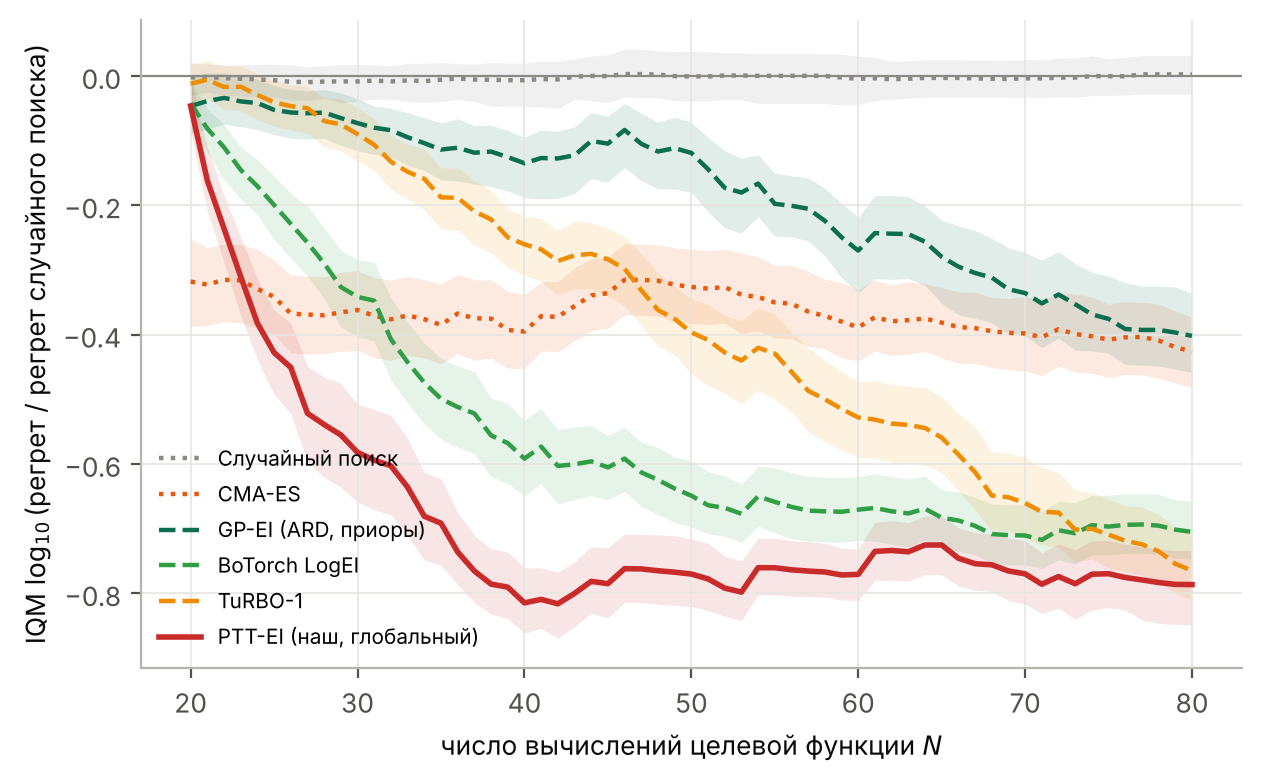
\includegraphics[width=\linewidth]{e9_anytime.png}
\end{column}
\begin{column}{0.40\textwidth}
\small 11 тестовых функций, $d=6$--$12$, 10 сидов. Ось $y$~--- $\log_{10}$ регрета относительно случайного поиска (меньше~--- лучше).
\vspace{0.4em}
\begin{itemize}\setlength\itemsep{3pt}
\item после 40 вычислений PTT-EI лучше всех: $-0.82$ против $-0.59$ у LogEI и $-0.26$ у TuRBO
\item затем PTT застревает, к 100 вычислениям TuRBO впереди ($-0.98$ против $-0.86$)
\item выигрыш не связан с TT-рангом функции; работает ANOVA-приор
\end{itemize}
\end{column}
\end{columns}
\end{frame}

\begin{frame}{Улучшение и проверка на новых задачах}
\begin{columns}[T]
\begin{column}{0.58\textwidth}
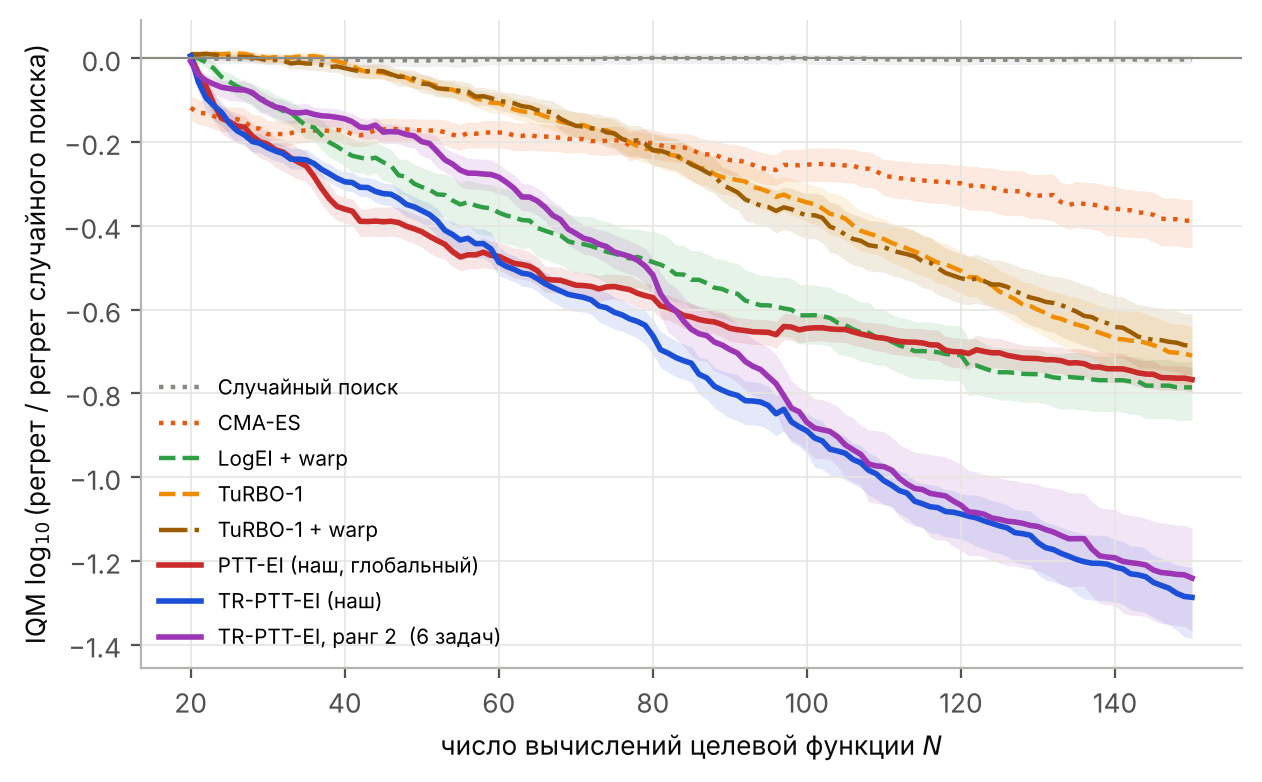
\includegraphics[width=\linewidth]{e14_anytime.png}
\end{column}
\begin{column}{0.40\textwidth}
\small TR-PTT: локальная PTT в доверительной области (правила TuRBO). Проверка на 9 задачах, не использованных при разработке ($d=10$--$20$); протокол записан до запуска.
\vspace{0.4em}
\begin{itemize}\setlength\itemsep{3pt}
\item TR-PTT $-1.39$, TuRBO $-0.80$, LogEI $-0.82$
\item лучше TuRBO в 75 из 90 пар, $p=2\cdot10^{-10}$
\item лучше и на раннем этапе: 81 из 90 пар
\end{itemize}
\vspace{0.4em}
{\color{muted}Дальше: реальные задачи, $d\ge 50$, дискретные переменные.}
\end{column}
\end{columns}
\end{frame}

\end{document}
